\begin{itemize}
    \item Parsec (pc) - disrance at which 1AU subtends an angle of 1 arcsecond
    \item Parallax - the apparent shift of a nearby star against distant background stars due to Earth's orbital motion. Used to measure stellar distances
    \item Proper motion - the angular motion of a star across the sky (per year), exclusding parallax
    \item Luminosity -  the total energy output of an object per unit time
    \item Brightness (Flux) - How bright an object appears from Earth
    \begin{equation*}
        F = \frac{L}{4 \pi d^2}
    \end{equation*}
    \item Magnitude - a logarithmic measure of brightness:
    \begin{itemize}
        \item Apparent magnitude (m) - how bright the object looks from Earth
        \begin{equation*}
            m_2 - m_1 = -2.512 \log \left( \frac{F_2}{F_1} \right)
        \end{equation*}
        \item absolute magnitude (M) - brightness at a standard distance of 10 pc
    \end{itemize}
    \item Effective temperature ($T_{\rm eff}$) Defined via $F = \sigma T^{4}_{\rm eff}$. Temperature that a blackbody would emit the same total radiation as the star. It determines stellar color and spectral type.
    \item Spectral Class - Classification of stars by their spectra and temperature:
    \begin{equation*}
        \text{O-B-A-F-G-K-M}
    \end{equation*}
    from hottest to coolest. Reflects surface temperature and ionization states of elements. mnemonic "Oh be a fine girl, kiss me"

    \item Hertzburgf-Russell diagram (HR-diagram) - a plot of luminosity vs temperature (of spectral class)
    \begin{center}
        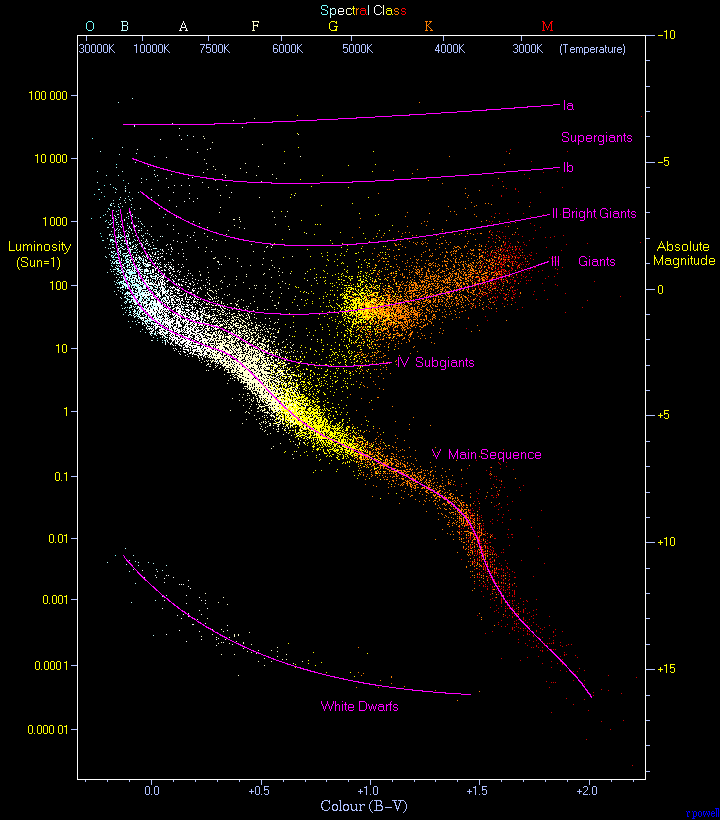
\includegraphics[width = 300pt]{images/HRDiagram.png}
    \end{center}

    \item Colour-Magnitude diagarm (CM-diagram) - observational version of HRD (magnitude vs color index). Used heavily for star-clusters, since distance is common
    \begin{center}
        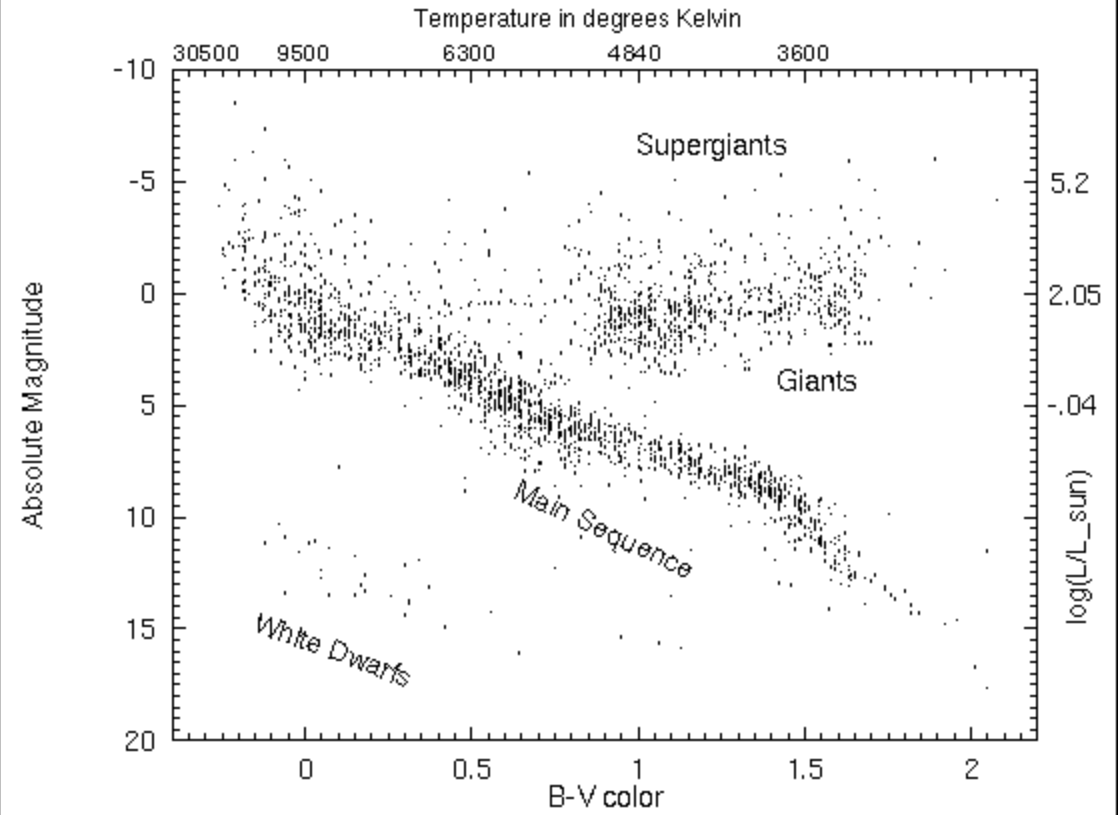
\includegraphics[width=300pt]{images/B-V diagram.png}
    \end{center}

    \item Kiel Diagram -  a theoretical evolution diagram (effective temperature vs surface gravity (log g))
    \begin{center}
        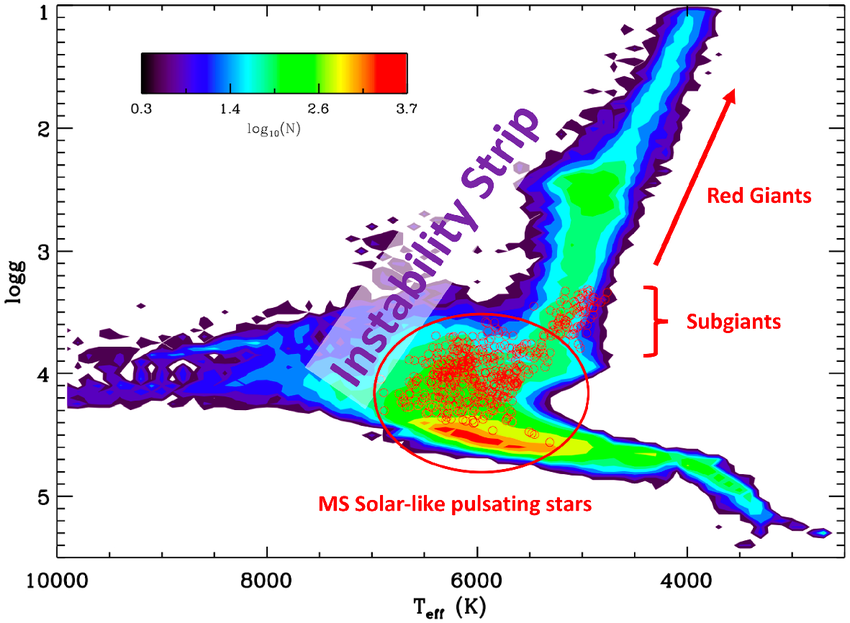
\includegraphics[width=300pt]{images/kiel diagram.png}
    \end{center}

    \item Kippenhahn diagram - a time-interior diagram of a star: shows convective vs radiative zones, nuclear burning regions, evolution of stellar structure over time
    \begin{center}
        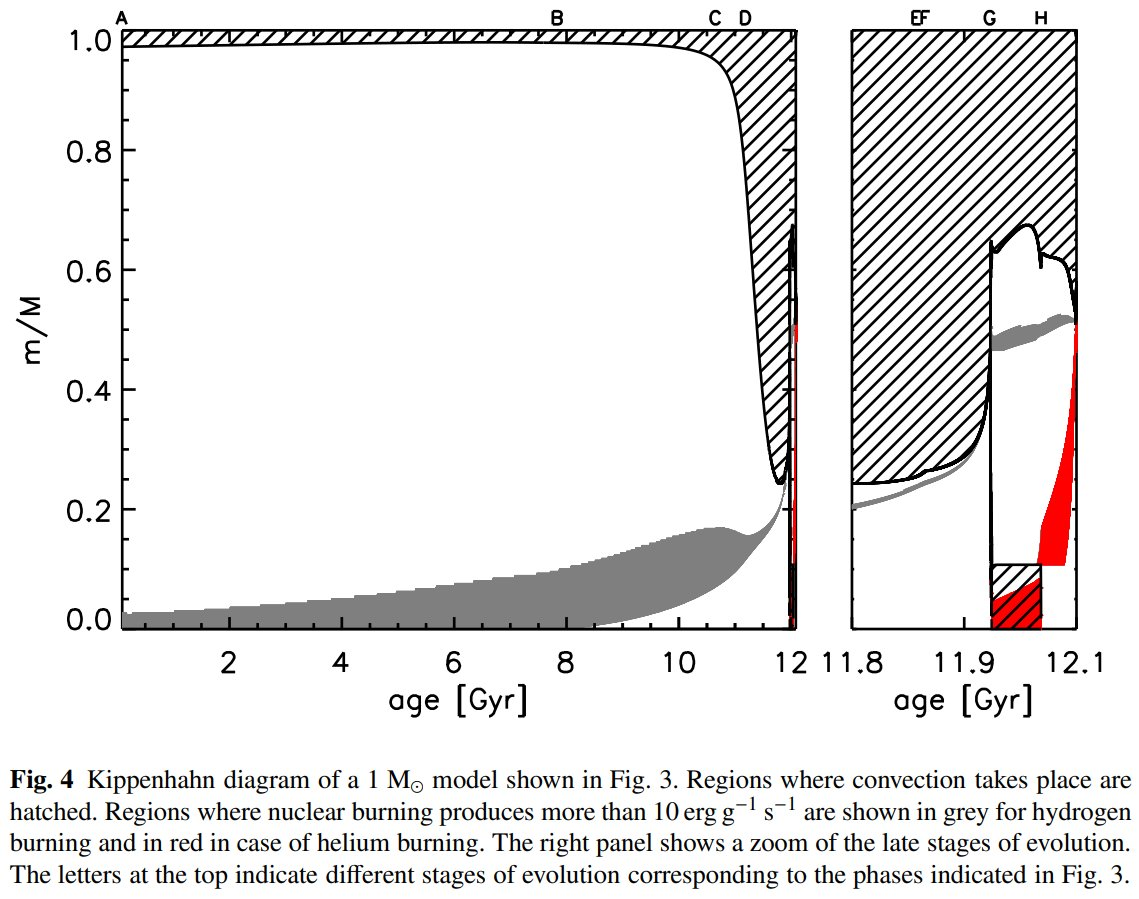
\includegraphics[width=300pt]{images/kippenhahn diagram.jpg}
    \end{center}

    \item Tc-$\rho$c diagram - a plot of central temperature $T_c$ vs central density $\rho_c$. Tracks internal evolution of a star, especially during late stages.
    \begin{center}
        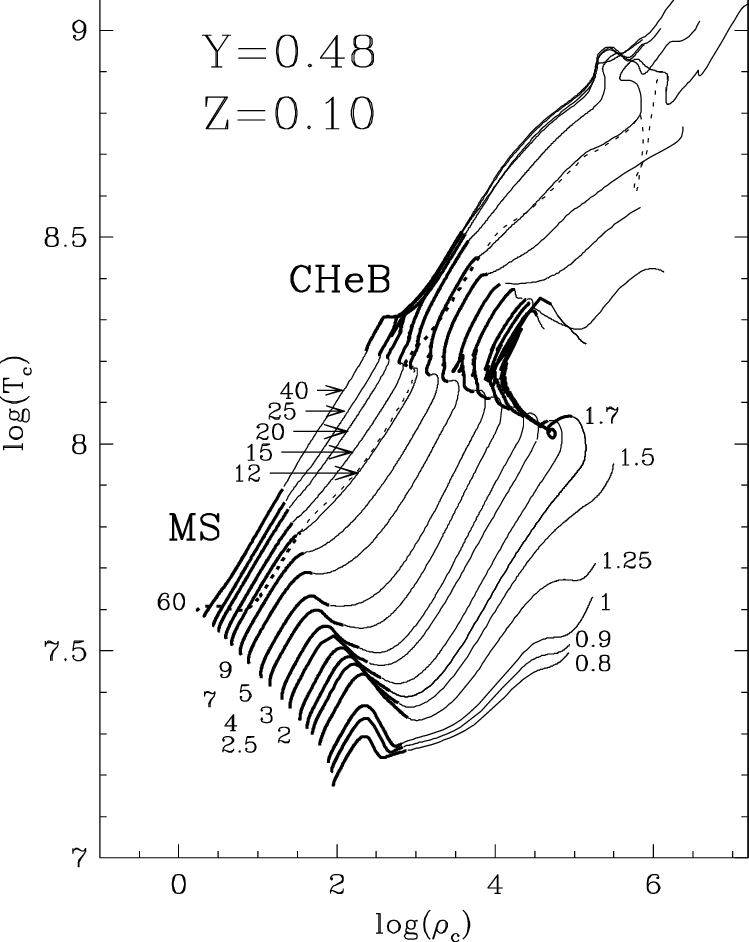
\includegraphics[width=300pt]{images/tc rhoc diagram.png}
    \end{center}

    \item Distance modulus - relates apparent and absolute magnitude
    \begin{equation*}
        m - M = 5 \log_{10}(d/pc) - 5
    \end{equation*}
    Used to determine distances when luminosity is known.

    \item Bolometric correction - Adjustment converting a magnitude ina given band (e.g. V) a total (bolometric) luminosity. Hot stars (blue) emit a lot of their radiation in ultraviolet, while cool stars (red) emit their radiation in infrared, is we only measure V (visible) band then we miss a lot radiation hence the bolometric correction. 
    
    \item Hydristatic equilibrium (HE) - the condition that keeps a star from collapsing or exploding. At every radius, inward gravity is balanced by outward preddure gradients:
    \begin{equation*}
        \frac{dP}{dr} = - \frac{G M(r) \rho(r)}{r^2}
    \end{equation*}
    
    \item Equation of state (EOS) - relates pressure, density and temperature\
    \begin{equation*}
        P = P (\rho, T, {\rm composition})
    \end{equation*}
    For example, ideal gas:
    \begin{equation*}
        P = \frac{\rho k_B T}{\mu m_{H}}
    \end{equation*}
    or a degenerate electron gas (white dwarfs). The EOS determines how a star responds to compression or heating.

    \item Virial theorem. Connects total gravitational energy $U$ and thermal energy $K$:
    \begin{equation*}
        2K + U = 0
    \end{equation*}
    Consequences: stars have negative total energy, when a star looses energy, it heats up.

    \item Energy transport -  how energy moves from the core to the surface
    \begin{itemize}
        \item Radiation: Energy carried by photons
        \begin{equation*}
            \frac{dT}{dr} = - \frac{3 \kappa \rho L}{16 \pi a c T^3 r^2}
        \end{equation*}

        \item Convection - Bulk motion of gas when radiation is inefficient. Occurs when:
        \begin{equation*}
            \Nabla_{\rm rad} > \Nabla_{\rm ad}
        \end{equation*}

        \item Conduction. Important only in very dense objects (white dwarfs, neutron stars)
    \end{itemize}

    \item Edington Equation (Edington Luminosity) - Maximum luminosity before radiation pressure overcomes gravity
    \begin{equation*}
        L_{\rm Edd} = \frac{4 \pi G M c}{\kappa}
    \end{equation*}

    If $L > L_{\rm Edd}$ material is blown away by radiation, which is important for massive stars and accretion disks.

    \item Opacity ($\kappa$) measures how opaque stellar material is to radiation. Sources being electron scattering, bound-free absorption, free-free absorption. Controls how efficiently radiation transports energy.
    
    \item Rosseland mean opacity -  aweighted average opacity used in radiative diffusion. Appropriate when radiation is close to equilibrium.
    
    \item Mixing length theory - a simplified model of stellar convection. Assumes fluid elements rise a distance $l = \alpha H_{P}$ where $H_P = \frac{P}{\rho g}$ is pressure scale height and $\alpha$ is a free parameter. MLT provides convective flux and temperature gradients.
    
    \item Thermohaline mixing - a double-diffusive instability, similar to salt fingers in oceans. It occurs when heavier material lies above lighter material, temperature stratification stabilizesm composition destabilizes. Important in red giants after nuclear burning alters composition.
    
    \item Diffusive mixing - gradual mixing treated as a diffusion process
    
    \item Semiconvection
    
    \item Magnetic fields in stars is generated by dynamo action: rotation + convection. The effects being modified energy transport, influence angular moimentum evolution, produce activity (spots, flares). Strong fields can suppress convection locally.
    
    \item Pre-main sequence (PMS) the phase where a star forms and contracts before hydrogen fusion begins. Energy source - gravitational contraction, star moves down and left in the HR diagram (Kelvin-Helmholtz timescale)
    
    \item Main sequence (MS) - The longest and most stable phase of stellar life.
    
    \item Zero-age main sequence (ZAMS) - The point where a star just begins stable hydrogen burning. Starting point for MS evolution tracks
    
    \item Overshooting - General term for mixing beyond formal convective boundaries
\end{itemize}